\documentclass[10pt]{scrartcl}

\usepackage{a4}
\usepackage{ngerman}
\usepackage[T1]{fontenc}
\usepackage[utf8]{inputenc}

\usepackage{calligra}
\usepackage{yfonts}

\usepackage{fancybox}

\usepackage[pdftex]{graphicx}

% \usepackage{url}
\usepackage{hyperref}


\title{ {\calligra Der Goldene Schnitt}}
\author{Wikipedia - {\small \url{http://de.wikipedia.org/wiki/Goldener_Schnitt}}}
\date{}

\begin{document}

\maketitle	

% Einfügen des Inhaltsverzeichnisses
\newpage
\setcounter{tocdepth}{2}
\renewcommand\contentsname{Inhaltsverzeichnis}
\tableofcontents

\newpage
\section{Einleitung}
\label{sec:Einleitung}

{\LARGE {\swabfamily{D}}}er \textbf{Goldene Schnitt} ist ein bestimmtes Verhältnis zweier Zahlen. Es beträgt etwa \texttt{1,618:1}.
Streckenverhältnisse im Goldenen Schnitt werden in der Kunst und Architektur oft als ideale Proportion und als Inbegriff von Ästhetik und Harmonie angesehen.

\begin{itemize}
	\item Das Seitenverhältnis \textbf{$\Phi$} beim Goldenen Schnitt ist eine \textbf{irrationale Zahl}, das heißt, sie lässt sich nicht durch ein Verhältnis zweier ganzer Zahlen darstellen. 
\item Subtrahiert man die kürzere der beiden Strecken von der längeren, so erhält man eine noch kürzere Strecke, zu der die mittlere der drei Strecken wiederum im Verhältnis des Goldenen Schnittes steht.
\end{itemize}

\section{Papier- und Bildformate}
\label{sec:PapierUndBildformate}

Im Buchdruck wurde früher gelegentlich die Nutzfläche einer Seite, 
der so genannte \textsc{Satzspiegel}, so positioniert, dass das Verhältnis von Bundsteg zu Kopfsteg zu Außensteg zu Fußsteg sich wie \texttt{2:3:5:8} verhielt.
Diese Wahl von \emph{Fibonacci-Zahlen} approximiert den Goldenen Schnitt.

Typische Einsatzgebiete der obigen prominenten Seitenverhältnisse lauten:

\begin{table}[htb]
\begin{center}

\begin{tabular} { | c | l|}
\hline
\textbf{Seitenverhältnis}   & \textbf{Einsatzgebiet}   \\ \hline
4 : 3              & Traditionelles Fernsehformat   \\ \hline
$\sqrt{2} : 1$     & Seitenverhältnis beim DIN-A4-Blatt \\   \hline
$16: 9 $            & Seitenverhältnis beim neuen Fernsehformat \\ 
\hline

\end{tabular}
	\caption{Einsatzgebiete}
	\label{tab:Einsatzgebiete}
\end{center}
\end{table} 

\section{Tabellen}
\label{sec:Tabellen}

Die Werte für $\Phi$ und $\pi$ lauten:

\begin{table}[htb]
\begin{center}
\begin{tabular} { | l | c|}
\hline
Symbol & Wert   \\ \hline
$\Phi$ & 1,61   \\
$\pi$ & 3,14    \\ \hline
\end{tabular}
	\caption{Symbole und Werte}
	\label{tab:SymboleUndWerte}
\end{center}
\end{table} 

\section{Geschichte}

Spaeter beschäftigte sich der Franziskanermoench Luca Pacioli di Borgo San Sepolcro (1445–1514), der an der Universität von Perugia Mathematik lehrte, mit Euklids Arbeiten.

 Er nannte diese Streckenteilung Goettliche Teilung, was sich auf Platons Identifizierung der Schoepfung mit den fuenf platonischen Koerpern bezog, zu deren Konstruktion der Goldene Schnitt ein wichtiges Hilfsmittel darstellt. Sein gleichnamiges Werk „De Divina Proportione“ von 1509 besteht aus drei unabhaengigen Buechern. 
 
Bei dem ersten handelt es sich um eine rein mathematische Abhandlung, die jedoch keinerlei Bezug zur Kunst und Architektur herstellt. 
 
Das zweite ist ein kurzer Traktat über die Schriften des Römers Vitruv aus dem 1. Jahrhundert v. Chr. zur Architektur, in denen Vitruv die Proportionen des menschlichen Körpers als Vorlage für Architektur darstellt. Dieses Buch enthält eine Studie von Leonardo da Vinci (1452-1519) über den vitruvianischen Menschen. Das Verhältnis von Quadratseite zu Kreisradius in diesem berühmten Bild (vgl. Abbildung \ref{fig:441px-Da_Vinci_Vitruve_Luc_Viatour} auf Seite \pageref{fig:441px-Da_Vinci_Vitruve_Luc_Viatour} entspricht mit einer Abweichung von 1,7\% dem Goldenen Schnitt, der jedoch im zugehörigen Buch gar nicht erwähnt wird. Darüber hinaus würde man diese Abweichung bei einem konstruktiven Verfahren nicht erwarten.

\begin{figure}[!htbp]
	\centering
	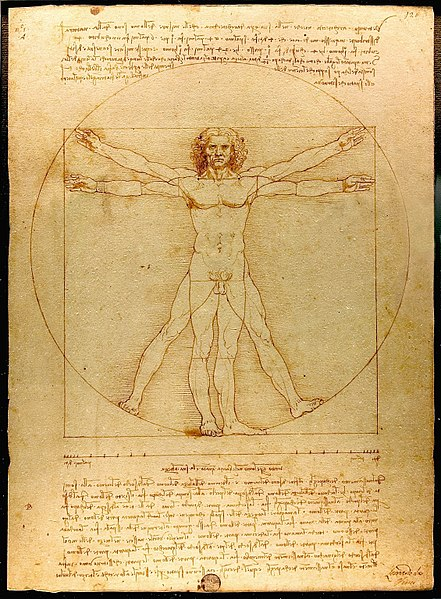
\includegraphics[width=0.75\textwidth]{441px-Da_Vinci_Vitruve_Luc_Viatour.jpg}
	\caption{Leonardo da Vinci: Der vitruvianische Mensch}
	\label{fig:441px-Da_Vinci_Vitruve_Luc_Viatour}
\end{figure}


\section{Herleitung des Zahlenwertes}
\label{sec:HerleitungDesZahlenwertes}


% Einfügen des Verzeichnisses der Tabellen
\newpage
\renewcommand\listtablename{Verzeichnis der verwendeten Tabellen}
\listoftables

% Einfügen des Verzeichnisses der Abbildungen
\newpage
\renewcommand\listfigurename{Verzeichnis der verwendeten Abbildungen}
\listoffigures
 
% Ende des Dokumentes
\end{document}